\section{问题三：烘干时间}

\subsection{问题分析}

第三问要求确定药材各处含水率均低于 $0.15\,\mathrm{kg/kg}$ 的烘干时间。该问与第二问具有相同的几何、物性关系和热湿耦合方程，因此沿用式~\eqref{eq:q2-pde}、\eqref{eq:q2-ibvp}，将计算时间延长至满足干燥要求。由于内部失水滞后于表面，\textbf{终止条件应由全域最大含水率确定}。

附件~1 给出的环境数据覆盖前 $4\,\mathrm h$。最后一小时的温度和环境水分浓度均值分别为 $49.9989\,{}^\circ\mathrm C$ 和 $0.0499875\,\mathrm{kg/kg}$，说明观测末段已经接近题设稳定工况。据此，前 $4\,\mathrm h$ 继续采用附件数据的分段线性插值，此后取

\begin{equation}
  T_\infty=50\,{}^\circ\mathrm C,\qquad
  C_\infty=0.05\,\mathrm{kg/kg}.
  \label{eq:q3-long-boundary}
\end{equation}

式~\eqref{eq:q3-long-boundary} 是第三问的长期边界条件，后文给出的烘干时间均以该工况持续保持为前提。

\subsection{终点判定}

记药材内部最大含水率为 $M(t)$，临界烘干时间 $t_d$ 定义为

\begin{equation}
  \left\{
  \begin{aligned}
    M(t)&=\max_{0\le r\le R_0}C(r,t),\\
    t_d&=\inf\left\{t\ge0:M(t)\le0.15\right\}.
  \end{aligned}
  \right.
  \label{eq:q3-end-time}
\end{equation}

其中 $R_0=0.02\,\mathrm m$，$C$ 的单位为 $\mathrm{kg/kg}$。临界状态满足 $M(t_d)=0.15$；继续干燥后，药材各处含水率严格低于阈值。

计算结果显示，在整个烘干过程中，药材含水率均由圆心向表面逐渐降低，最大含水率始终出现在圆心。因此，\textbf{圆心是最后达到干燥要求的位置}，式~\eqref{eq:q3-end-time} 可进一步化为

\begin{equation}
  M(t)=C(0,t),\qquad C(0,t_d)=0.15.
  \label{eq:q3-center-event}
\end{equation}

\subsection{模型求解}

沿用第二问的守恒空间离散和 BDF 自适应积分，联立推进温度场与含水率场。在积分过程中监测

\[
  g(t)=C(0,t)-0.15
\]

的首次下降过零，并利用连续插值定位 $t_d$。随后以全域最大含水率复核终点，确认临界点前尚未全部达标，临界点后已严格低于阈值。完整结果按 $60\,\mathrm s$ 的时间间隔和 $0.1\,\mathrm{cm}$ 的空间间隔保存，论文结果表的末行直接取临界状态。

\subsection{结果分析}

在 $4\,\mathrm h$ 后持续满足式~\eqref{eq:q3-long-boundary} 的条件下，药材全域含水率首次达到规定阈值的时间为

\[
  \boxed{t_d\approx57.4722\,\mathrm h}.
\]

该数值按题目要求保留四位小数。每隔 $6\,\mathrm h$ 及临界时刻的含水率见表~\ref{tab:q3-moisture}。

\begin{table}[H]
  \centering
  \caption{药材烘干过程的水分浓度（$\mathrm{kg/kg}$）}
  \label{tab:q3-moisture}
  \begin{tabular}{rrrrrr}
    \toprule
    时间/h & $0\,\mathrm{cm}$ & $0.5\,\mathrm{cm}$ & $1\,\mathrm{cm}$ & $1.5\,\mathrm{cm}$ & $2\,\mathrm{cm}$ \\
    \midrule
    6       & 1.0170 & 0.9881 & 0.9015 & 0.7550 & 0.5328 \\
    12      & 0.4561 & 0.4432 & 0.4031 & 0.3297 & 0.1642 \\
    18      & 0.2988 & 0.2915 & 0.2687 & 0.2253 & 0.0845 \\
    24      & 0.2378 & 0.2327 & 0.2167 & 0.1855 & 0.0665 \\
    30      & 0.2058 & 0.2018 & 0.1892 & 0.1641 & 0.0598 \\
    36      & 0.1859 & 0.1825 & 0.1718 & 0.1504 & 0.0566 \\
    42      & 0.1721 & 0.1691 & 0.1597 & 0.1407 & 0.0549 \\
    48      & 0.1618 & 0.1592 & 0.1507 & 0.1334 & 0.0537 \\
    54      & 0.1539 & 0.1514 & 0.1436 & 0.1277 & 0.0530 \\
    57.4722 & 0.1500 & 0.1477 & 0.1402 & 0.1249 & 0.0527 \\
    \bottomrule
  \end{tabular}
\end{table}


临界时刻，圆心含水率为 $0.1500\,\mathrm{kg/kg}$，表面已降至 $0.0527\,\mathrm{kg/kg}$。表面约在 $12.55\,\mathrm h$ 达到阈值，圆心则在 $57.47\,\mathrm h$ 最后达标，两者相差约 $44.92\,\mathrm h$。可见，表面含水率较早降至阈值时，药材内部仍未满足烘干要求，因而\textbf{表面状态不能代表药材整体的干燥程度，实际停机时刻应由圆心含水率确定}。

\subsection{结果可靠性检验}

临界烘干时间是本问的核心结果。为考察其是否依赖径向网格的划分尺度，在其余条件不变的情况下，分别取 2560、5120 和 10240 个径向区间进行计算，结果见表~\ref{tab:q3-convergence}。

\begin{table}[H]
  \centering
  \fontsize{10.5pt}{12.6pt}\selectfont
  \renewcommand{\arraystretch}{1.25}
  \captionsetup{font=small,labelfont=bf,textfont=bf}
  \caption{临界烘干时间的网格收敛}
  \label{tab:q3-convergence}
  \begin{tabularx}{0.82\textwidth}{|>{\centering\arraybackslash}X|>{\centering\arraybackslash}X|>{\centering\arraybackslash}X|>{\centering\arraybackslash}X|}
    \hline
    网格等级 & 区间数 $N$ & 达标时间/h & 相邻差异/s \\
    \hline
    粗 & 2560  & 57.471395 & --- \\
    \hline
    中 & 5120  & 57.472066 & 2.42 \\
    \hline
    细 & 10240 & 57.472244 & 0.64 \\
    \hline
  \end{tabularx}
\end{table}


由表可见，网格逐级加密时，临界烘干时间趋于稳定，其中 5120 个区间加密至 10240 个区间后，终点仅变化 $0.64\,\mathrm s$。在细网格上进一步收紧时间积分容差并减小最大步长，所得终点又仅变化 $0.0129\,\mathrm s$。空间和时间两方面的比较均表明，\textbf{现有离散精度足以支撑 $57.4722\,\mathrm h$ 的终点判断}。此外，含水率总量变化与表面传质通量之间的最大相对平衡残差为 $5.32\times10^{-7}$，说明离散求解较好地保持了质量守恒。

\subsection{长期工况敏感性}

由于超过九成的预测时段位于环境观测窗口之外，长期边界是影响终点解释的重要假设。保持前 $4\,\mathrm h$ 的附件数据不变，只改变此后的恒定工况，结果见图~\ref{fig:q3-boundary-sensitivity}。

\begin{figure}[H]
  \centering
  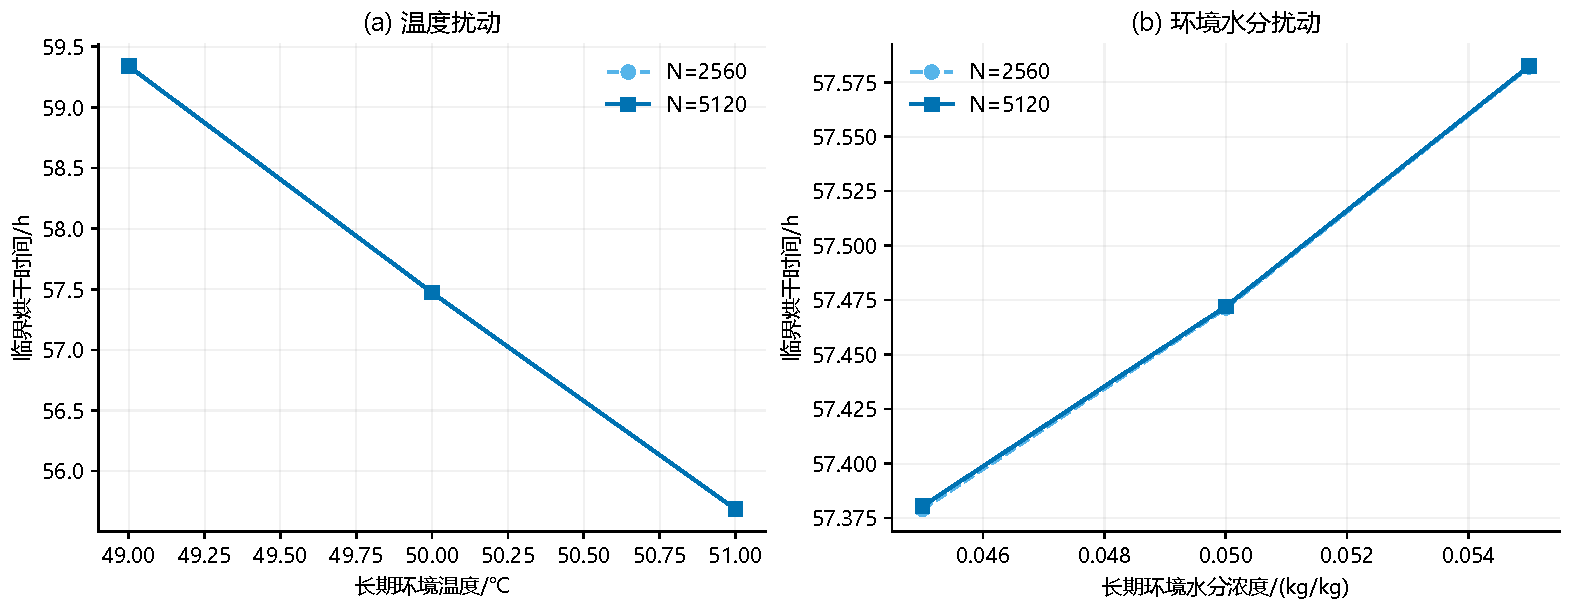
\includegraphics[width=0.96\textwidth]{figures/q3_boundary_sensitivity.pdf}
  \caption{长期环境条件对临界烘干时间的影响}
  \label{fig:q3-boundary-sensitivity}
\end{figure}

长期温度取 $49$、$50$ 和 $51\,{}^\circ\mathrm C$ 时，临界时间分别为 $59.3392$、$57.4721$ 和 $55.6865\,\mathrm h$；相对基准工况，温度降低 $1\,{}^\circ\mathrm C$ 使烘干时间延长 $1.867\,\mathrm h$，温度升高 $1\,{}^\circ\mathrm C$ 则使其缩短 $1.786\,\mathrm h$。当环境水分浓度取 $0.045$、$0.050$ 和 $0.055\,\mathrm{kg/kg}$ 时，临界时间分别为 $57.3804$、$57.4721$ 和 $57.5824\,\mathrm h$，变化约为 $-0.09$ 至 $0.11\,\mathrm h$。

因此，在所考察的扰动范围内，\textbf{温度变化造成的终点偏移明显大于环境水分浓度变化}，表明最终达标时间对这组长期温度扰动更敏感。这进一步说明，$57.4722\,\mathrm h$ 是长期环境维持基准工况时的条件预测，而不是脱离运行条件的固定时长。图中的扰动范围用于比较给定工况，不代表未来环境的统计置信区间。

\subsection{后期干燥长尾的形成}

为解释圆心达标明显滞后的原因，将各时刻的温度和含水率代入扩散系数关系，得到圆心、$r=0.5R_0$ 和表面的有效扩散系数变化，如图~\ref{fig:q3-diffusivity} 所示。

\begin{figure}[H]
  \centering
  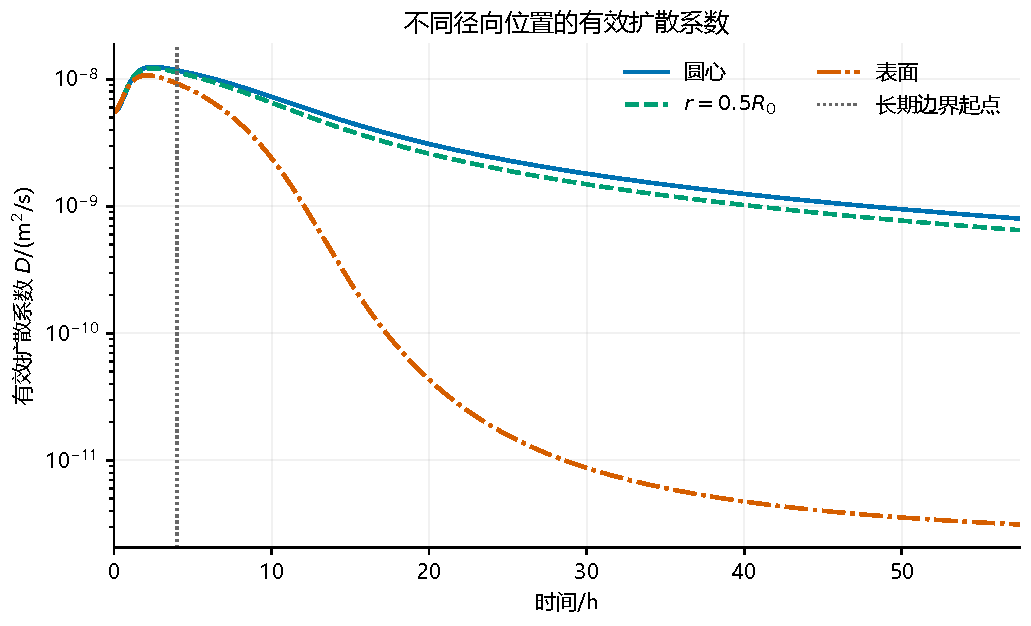
\includegraphics[width=0.86\textwidth]{figures/q3_diffusivity.pdf}
  \caption{不同径向位置的有效扩散系数随时间的变化}
  \label{fig:q3-diffusivity}
\end{figure}

图~\ref{fig:q3-diffusivity} 显示，升温初期三个位置的扩散系数均有所增大；温度逐渐稳定后，含水率下降的影响开始占据主导，扩散系数随之减小。由于表层最先失水，其扩散系数也最早、最快下降，并逐渐与内部曲线拉开差距。到临界时刻，圆心和表面的扩散系数分别约为 $8.00\times10^{-10}\,\mathrm{m^2/s}$ 和 $3.12\times10^{-12}\,\mathrm{m^2/s}$，前者约为后者的 256 倍。

这说明药材在后期并非均匀干燥：外层含水率降低后，逐渐形成扩散能力较弱的区域，而圆心附近仍保留较多水分。内部水分向外迁移时需要经过这一低扩散区域，使后期失水速度不断减缓。因此，表面在 $12.55\,\mathrm h$ 达标后，圆心仍需较长时间才能降至阈值，最终形成从 $12.55\,\mathrm h$ 延续至 $57.47\,\mathrm h$ 的干燥长尾。\textbf{第三问较长的终点时间，反映的正是内部剩余水分缓慢向外迁移的过程。}这里的 256 倍用于说明扩散能力的径向差异；实际传质速率仍由扩散系数和含水率梯度共同决定。
